%==============================================================================
%  Mycellium-Aegis — AI & Signal-Intelligence Plan
%  Beamer presentation (companion to Mycellium-Aegis_AI_Plan_APA7.md)
%
%  Compile:  pdflatex -interaction=nonstopmode Mycellium-Aegis_AI_Plan_Beamer.tex
%            (run twice so the section/frame counters settle)
%
%  Self-contained: only standard TeX Live packages (beamer, tikz, booktabs,
%  xcolor, lmodern, appendixnumberbeamer). No external images or fonts.
%==============================================================================
\PassOptionsToPackage{table}{xcolor}
\documentclass[aspectratio=169,11pt]{beamer}

\usepackage[T1]{fontenc}
\usepackage[utf8]{inputenc}
\usepackage{lmodern}
\usepackage{booktabs}
\usepackage{tikz}
\usepackage{appendixnumberbeamer}
\usetikzlibrary{arrows.meta,positioning,shapes.geometric,calc}

%------------------------------------------------------------------ colours ---
\definecolor{aegisGreen}{HTML}{2E7D32}
\definecolor{aegisDark}{HTML}{1B5E20}
\definecolor{aegisLeaf}{HTML}{4E8A3A}
\definecolor{aegisAI}{HTML}{6A1B9A}
\definecolor{aegisBlue}{HTML}{0277BD}
\definecolor{aegisInk}{HTML}{233329}
\definecolor{aegisMist}{HTML}{EAF1EA}
\definecolor{aegisAmber}{HTML}{C77800}

%------------------------------------------------------------------- theme ----
\usetheme{default}
\usecolortheme{default}
\setbeamercolor{normal text}{fg=aegisInk}
\setbeamercolor{structure}{fg=aegisGreen}
\setbeamercolor{frametitle}{fg=white,bg=aegisDark}
\setbeamercolor{title}{fg=aegisDark}
\setbeamercolor{alerted text}{fg=aegisAmber}
\setbeamercolor{block title}{fg=white,bg=aegisGreen}
\setbeamercolor{block body}{fg=aegisInk,bg=aegisMist}
\setbeamercolor{itemize item}{fg=aegisLeaf}
\setbeamercolor{itemize subitem}{fg=aegisLeaf}
\setbeamercolor{section in toc}{fg=aegisInk}

\setbeamerfont{frametitle}{series=\bfseries}
\setbeamerfont{title}{series=\bfseries,size=\LARGE}
\setbeamertemplate{navigation symbols}{}
\setbeamertemplate{itemize items}[circle]
\setbeamertemplate{blocks}[rounded][shadow=false]

% frame title as a full-width band
\setbeamertemplate{frametitle}{%
  \nointerlineskip
  \begin{beamercolorbox}[wd=\paperwidth,ht=3.1ex,dp=1.2ex,leftskip=0.6cm,rightskip=0.6cm]{frametitle}%
    \usebeamerfont{frametitle}\insertframetitle%
  \end{beamercolorbox}%
}

% slim footline
\setbeamertemplate{footline}{%
  \leavevmode\hbox{%
    \begin{beamercolorbox}[wd=.34\paperwidth,ht=2.4ex,dp=1ex,leftskip=.3cm]{author in head/foot}%
      \color{aegisDark}\footnotesize Mycellium-Aegis%
    \end{beamercolorbox}%
    \begin{beamercolorbox}[wd=.5\paperwidth,ht=2.4ex,dp=1ex,center]{title in head/foot}%
      \color{aegisInk}\footnotesize AI \& Signal-Intelligence Plan%
    \end{beamercolorbox}%
    \begin{beamercolorbox}[wd=.16\paperwidth,ht=2.4ex,dp=1ex,rightskip=.3cm]{date in head/foot}%
      \hfill\color{aegisDark}\footnotesize\insertframenumber\,/\,\inserttotalframenumber%
    \end{beamercolorbox}}%
}

% section divider slides
\AtBeginSection[]{%
  \begin{frame}[plain]
    \centering
    \vfill
    {\color{aegisLeaf}\rule{2.2cm}{2pt}}\\[0.6em]
    {\usebeamerfont{title}\color{aegisDark}\insertsectionhead}\\[0.4em]
    {\color{aegisLeaf}\rule{2.2cm}{2pt}}
    \vfill
  \end{frame}
}

% handy macro for a small caption line
\newcommand{\src}[1]{{\scriptsize\color{aegisLeaf}#1}}

%------------------------------------------------------------------- meta -----
\title{Artificial Intelligence \& Signal-Intelligence Plan}
\subtitle{An LSTM Sensor-Fusion Approach to Pre-Ignition Wildfire Detection\\ from Mycelial Bioelectric Activity}
\author{Muhammet Yağcıoğlu \and Mehmet Çetin \and Ömer Ünal \and Mahmut Can Göçlü}
\institute{Mycellium-Aegis \,·\, İzmir Institute of Technology (İYTE) Teknopark\\ TÜBİTAK 1812 BİGG \,·\, Green Growth}
\date{2026}

%==============================================================================
\begin{document}

%------------------------------------------------------------- title slide ----
{%
\setbeamertemplate{footline}{}
\begin{frame}[plain]
  \vfill
  \begin{beamercolorbox}[wd=\paperwidth,sep=10pt,leftskip=0.8cm,rightskip=0.8cm]{block body}
    {\color{aegisLeaf}\footnotesize\bfseries LIVING MYCELIUM BIOSENSORS \,·\, PRE-IGNITION FOREST-FIRE EARLY WARNING}\\[0.7em]
    {\usebeamerfont{title}\color{aegisDark}\inserttitle}\\[0.5em]
    {\color{aegisInk}\insertsubtitle}
  \end{beamercolorbox}
  \vskip1.0em
  {\centering
    \color{aegisInk}\small\insertauthor\\[0.5em]
    {\footnotesize\color{aegisLeaf}\insertinstitute}\\[0.5em]
    {\footnotesize\color{aegisInk}\insertdate}\par}
  \vfill
  {\centering\scriptsize\color{aegisLeaf} Companion deck to the APA~7 written plan \texttt{(Mycellium-Aegis\_AI\_Plan\_APA7.md)}\par}
\end{frame}
}

%------------------------------------------------------------------ outline ---
\begin{frame}{Where we are going}
  \setbeamertemplate{section in toc}[sections numbered]
  \tableofcontents
\end{frame}

%==============================================================================
\section{The Problem}
%==============================================================================

\begin{frame}{Today's early-warning stack detects fire too late}
  Satellites, UAVs, camera towers and above-ground sensor networks all share one
  blind spot: they fire only \alert{after} flame, heat radiation or smoke exists.
  \vskip0.6em
  \begin{center}
  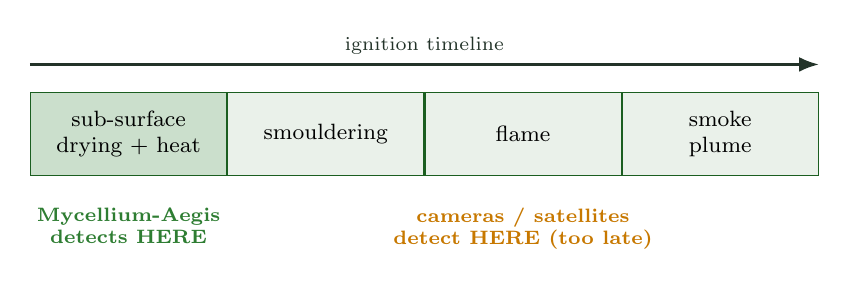
\begin{tikzpicture}[font=\footnotesize,node distance=0pt]
    \tikzset{phase/.style={draw=aegisDark,fill=aegisMist,minimum height=1.05cm,text width=2.35cm,align=center,inner sep=2pt}}
    \node[phase,fill=aegisGreen!25] (a) {sub-surface\\ drying + heat};
    \node[phase,right=of a] (b) {smouldering};
    \node[phase,right=of b] (c) {flame};
    \node[phase,right=of c] (d) {smoke\\ plume};
    \draw[-{Latex[length=2.5mm]},aegisInk,thick] ($(a.north west)+(0,0.35)$) -- ($(d.north east)+(0,0.35)$)
      node[midway,above,font=\scriptsize]{ignition timeline};
    \node[below=0.28cm of a,align=center,aegisGreen,font=\bfseries\scriptsize] {Mycellium-Aegis\\ detects HERE};
    \node[below=0.28cm of c,align=center,aegisAmber,font=\bfseries\scriptsize] {cameras / satellites\\ detect HERE (too late)};
  \end{tikzpicture}
  \end{center}
  \begin{block}{The shift}
    Move the detection window \emph{earlier} — to the pre-ignition stage — by
    monitoring sub-surface moisture loss and heat build-up that precede ignition.
  \end{block}
\end{frame}

\begin{frame}{The core idea: listen to the forest floor}
  \begin{columns}[T]
    \begin{column}{0.54\textwidth}
      Underground \structure{mycelial networks} produce reproducible, directional
      voltage \structure{spikes} in response to heat, drying and damage.
      \vskip0.4em
      At \textbf{15--20 cm} depth a $>900\,^\circ$C surface flame arrives as a
      damped $25$--$50\,^\circ$C wave: cool enough for the mycelium to survive and
      keep signalling, yet coupled to the surface.
      \vskip0.4em
      \src{Adamatzky (2018, 2026a, 2026b); Phillips et al.\ (2023); Doerr et al.\ (2025)}
    \end{column}
    \begin{column}{0.46\textwidth}
      \footnotesize
      \begin{tabular}{@{}r l@{}}
        \toprule
        \textbf{Depth} & \textbf{Effect on networks} \\
        \midrule
        0--2 cm  & near-total destruction \\
        2--5 cm  & partial; spores survive \\
        5--10 cm & pyrophilic fungi activate \\
        \rowcolor{aegisGreen!18}\textbf{15--20 cm} & \textbf{mycelium keeps sensing} \\
        \bottomrule
      \end{tabular}
      \vskip0.4em
      \src{The 15--20 cm ``safe zone'' is both survivable and measurable.}
    \end{column}
  \end{columns}
\end{frame}

\begin{frame}{Why this is fundamentally an \emph{AI} problem}
  The sensing is solved; the \alert{decision} is the risk. Each raw channel is
  individually ambiguous:
  \begin{itemize}
    \item a hot afternoon raises soil temperature,
    \item a long drought raises substrate resistance,
    \item background metabolism produces occasional spikes.
  \end{itemize}
  \vskip0.3em
  \begin{block}{Consequence}
    Any single channel, thresholded naively, produces false alarms that destroy
    operational trust and waste firefighting resources. The AI system exists to
    fuse weak, multi-rate signals into one \structure{low-false-alarm} decision.
  \end{block}
\end{frame}

%==============================================================================
\section{Objectives \& Success Criteria}
%==============================================================================

\begin{frame}{One headline commitment, measured}
  \begin{block}{Primary objective}
    Detect fire onset in the pre-ignition phase with a
    \alert{false-positive rate $<1\%$} while keeping recall high — because at
    hundreds--thousands of nodes, false alarms dominate operational trust.
  \end{block}
  \vskip0.2em
  \centering\footnotesize
  \begin{tabular}{@{}l l l@{}}
    \toprule
    \textbf{Objective} & \textbf{Metric} & \textbf{Target} \\
    \midrule
    Minimize false alarms & FPR & $<1\%$ (field-representative) \\
    Preserve sensitivity  & Recall & $\ge 0.95$ \\
    Balanced quality      & PR-AUC / F$_1$ & $\ge 0.98$ / $\ge 0.95$ \\
    Timeliness            & Latency & alarm before surface flame \\
    Edge feasibility      & Model / RAM & $\le 128$ KB / $\le 256$ KB \\
    Interpretability      & Baseline agreement & explainable vs.\ AND rule \\
    \bottomrule
  \end{tabular}
  \vskip0.4em
  \src{``Field-representative'' = includes drought, diurnal/seasonal swings and non-fire heating.}
\end{frame}

%==============================================================================
\section{Data Foundation}
%==============================================================================

\begin{frame}{Experiment 1 — the signature is in the \emph{frequency} domain}
  \begin{columns}[T]
    \begin{column}{0.55\textwidth}
      Single differential channel, \emph{Pleurotus ostreatus},
      $f_s\approx45$ Hz, raw (GAIN\_SIXTEEN, $7.81\,\mu$V/bit).
      \vskip0.5em
      \footnotesize
      \begin{tabular}{@{}l r r@{}}
        \toprule
         & \textbf{Resting} & \textbf{Fire stress} \\
        \midrule
        Mean voltage & $-2.9$ mV & $-2.94$ mV \\
        Min voltage  & $-29.4$ mV & $-33.4$ mV \\
        Dominant freq. & $\approx20$ Hz & $\approx5$ Hz \\
        Samples $N$ & 1{,}048 & 1{,}085 \\
        \bottomrule
      \end{tabular}
    \end{column}
    \begin{column}{0.45\textwidth}
      \begin{block}{Key result}
        Mean voltage barely moves — but the \structure{dominant band migrates
        $\approx20\to\approx5$ Hz} under heat stress.
      \end{block}
      A naive amplitude threshold fails; the \emph{spectral} and
      \emph{distributional} change carries the signal $\Rightarrow$ motivates
      sequence / spectro-temporal modelling.
    \end{column}
  \end{columns}
\end{frame}

\begin{frame}{Experiment 2 — toward field realism}
  Active soil--mycelium network, two channels, with real DSP.
  \vskip0.4em
  \centering\footnotesize
  \begin{tabular}{@{}l l l@{}}
    \toprule
    \textbf{Parameter} & \textbf{Experiment 1} & \textbf{Experiment 2} \\
    \midrule
    Subject      & single tissue & soil/mycelium network \\
    Channels     & 1 differential & \textbf{2 differential} (network map) \\
    PGA gain     & $\pm0.256$ V & $\pm6.144$ V (24$\times$ range) \\
    Sample rate  & $\approx45$ Hz & $\approx100$ Hz (Nyquist 50 Hz) \\
    Filtering    & none (raw) & 5-tap linear-phase FIR $[0.1,0.2,0.4,0.2,0.1]$ \\
    Offset cal.  & none & automatic (50-sample baseline) \\
    \bottomrule
  \end{tabular}
  \vskip0.5em
  \begin{columns}[T]
    \begin{column}{0.5\textwidth}
      \src{FIR: unity DC gain ($\sum h_k=1.0$), linear phase — denoises without
      distorting the derivatives.}
    \end{column}
    \begin{column}{0.5\textwidth}
      \src{Two channels map thermal-stress \emph{propagation}, not a single point.}
    \end{column}
  \end{columns}
\end{frame}

\begin{frame}{Labels, provenance \& class imbalance}
  \begin{columns}[T]
    \begin{column}{0.52\textwidth}
      \textbf{Four physical regimes} (not just alarm/no-alarm):
      \begin{itemize}
        \item \structure{normal} — diurnal/seasonal baseline
        \item \structure{drought} — slow drying, no heat inflow
        \item \structure{non-fire heating} — solar / sub-surface source
        \item \alert{fire onset} — heat $+$ rapid drying $+$ spiking
      \end{itemize}
      This is what lets the model learn \emph{drought vs.\ fire}.
    \end{column}
    \begin{column}{0.48\textwidth}
      \textbf{Imbalance} (onset is rare) handled at three levels:
      \begin{enumerate}
        \item collect — over-sample controlled onsets;
        \item resample — SMOTE on the \emph{train split only};
        \item physics-informed augmentation (time-warp, jitter, baseline wander, noise superposition).
      \end{enumerate}
      \src{Provenance versioned per datasheet discipline (Gebru et al., 2021).}
    \end{column}
  \end{columns}
\end{frame}

%==============================================================================
\section{Method}
%==============================================================================

\begin{frame}{Signal-processing \& feature pipeline}
  \centering
  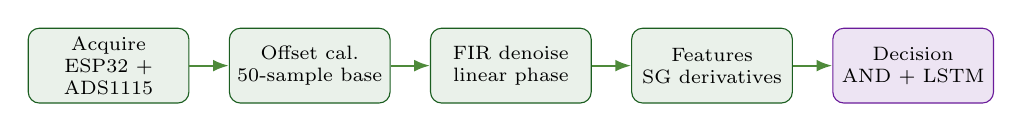
\begin{tikzpicture}[font=\scriptsize,node distance=0.42cm and 0.5cm,
      box/.style={draw=aegisDark,fill=aegisMist,rounded corners,minimum height=0.95cm,text width=1.9cm,align=center,inner sep=2pt},
      ai/.style={draw=aegisAI,fill=aegisAI!12,rounded corners,minimum height=0.95cm,text width=1.9cm,align=center,inner sep=2pt}]
    \node[box] (acq) {Acquire\\ ESP32 + ADS1115};
    \node[box,right=of acq] (off) {Offset cal.\\ 50-sample base};
    \node[box,right=of off] (fir) {FIR denoise\\ linear phase};
    \node[box,right=of fir] (feat) {Features\\ SG derivatives};
    \node[ai,right=of feat] (dec) {Decision\\ AND $+$ LSTM};
    \foreach \a/\b in {acq/off,off/fir,fir/feat,feat/dec}
      \draw[-{Latex[length=2mm]},aegisLeaf,thick] (\a) -- (\b);
  \end{tikzpicture}
  \vskip0.6em
  \begin{columns}[T]
    \begin{column}{0.5\textwidth}
      \textbf{Core fusion features}
      \begin{itemize}\footnotesize
        \item heat-flux rate \; $dT/dt$
        \item drying rate \; $d(\ln R)/dt$
        \item spike frequency \; $f_{\text{spike}}$
      \end{itemize}
    \end{column}
    \begin{column}{0.5\textwidth}
      \textbf{Spectral \& statistical}
      \begin{itemize}\footnotesize
        \item band-power ratio, spectral centroid, dominant freq.
        \item variance, skew, kurtosis, Hjorth
      \end{itemize}
    \end{column}
  \end{columns}
  \vskip0.2em
  \src{Savitzky--Golay (1964) smooths signal \emph{and} derivative in one pass.}
\end{frame}

\begin{frame}{A two-tier decision system}
  \begin{columns}[T]
    \begin{column}{0.5\textwidth}
      \begin{block}{Tier 1 — deterministic (safety floor)}
        \small
        \[ \text{Alarm}=(dT/dt>\beta)\ \wedge\ (d(\ln R)/dt>\gamma)\ \wedge\ \text{spike} \]
        Interpretable, near-zero compute, always available.
        $\beta,\gamma$ fixed at \textbf{98\%} confidence in a climate chamber.
      \end{block}
    \end{column}
    \begin{column}{0.5\textwidth}
      \begin{block}{Tier 2 — learned (LSTM)}
        \small
        Learns the \emph{joint temporal shape} the rigid AND rule ignores;
        outputs a calibrated probability with a \structure{tunable operating point}
        for FPR $<1\%$.
      \end{block}
    \end{column}
  \end{columns}
  \vskip0.4em
  \begin{block}{Escalation}
    High-severity alarm = LSTM probability over threshold \alert{AND} deterministic
    rule corroborates \alert{AND} neighbouring nodes agree. The interpretable rule
    stays in the loop; the model removes false alarms.
  \end{block}
\end{frame}

\begin{frame}{Model architecture — why recurrent}
  Fire onset is defined by how $dT/dt$, $d(\ln R)/dt$ and spike dynamics
  \emph{co-evolve} over seconds--minutes, plus the spectral migration. LSTMs learn
  temporal dependencies while mitigating vanishing gradients
  \src{(Hochreiter \& Schmidhuber, 1997)}.
  \vskip0.4em
  \textbf{Reference model (edge-bounded)}
  \begin{itemize}\small
    \item \textbf{Input:} windowed feature vector (fusion + spectral + statistical); optional raw channels.
    \item \textbf{Core:} 1--2 LSTM layers, 32--64 units; dropout regularizes the small-data regime.
    \item \textbf{Head:} 4-way softmax (normal / drought / non-fire heat / fire onset).
    \item \textbf{Calibration:} temperature scaling $\Rightarrow$ threshold controls FPR.
  \end{itemize}
  \src{Sized against the ESP32 budget, not for maximal accuracy.}
\end{frame}

\begin{frame}{The LSTM is a baseline, not a foregone conclusion}
  \centering\footnotesize
  \begin{tabular}{@{}l l l@{}}
    \toprule
    \textbf{Model family} & \textbf{Strength} & \textbf{Risk / fit} \\
    \midrule
    \rowcolor{aegisAI!12}\textbf{LSTM} (baseline) & long-range temporal & sequential; primary choice \\
    1D CNN & cheap, learns spectral motifs & weak long memory; strong front end \\
    CNN--LSTM hybrid & motifs $+$ evolution & larger; if either underfits \\
    TCN & long receptive field, parallel & newer MCU export (Bai et al., 2018) \\
    Transformer & global context & data-hungry; deferred (Vaswani et al., 2017) \\
    Gradient-boosted trees & robust tabular baseline & no native temporal model \\
    \bottomrule
  \end{tabular}
  \vskip0.5em
  \begin{block}{Selection rule}
    Whichever meets the targets at the \structure{lowest edge cost};
    interpretability breaks ties. All learned models are benchmarked against the
    deterministic rule \emph{and} a gradient-boosted-trees baseline.
  \end{block}
\end{frame}

\begin{frame}{Training methodology}
  \begin{columns}[T]
    \begin{column}{0.5\textwidth}
      \textbf{Honest splits}
      \begin{itemize}\small
        \item grouped, time-blocked CV
        \item leave-one-session-out (lab)
        \item leave-one-site-out (field)
        \item no window straddles a split $\Rightarrow$ no leakage
      \end{itemize}
      \vskip0.3em
      \textbf{Imbalance}
      \begin{itemize}\small
        \item class-weighted / focal loss (Lin et al., 2017)
        \item SMOTE on train split only (Chawla et al., 2002)
      \end{itemize}
    \end{column}
    \begin{column}{0.5\textwidth}
      \textbf{Optimization}
      \begin{itemize}\small
        \item Adam (Kingma \& Ba, 2015)
        \item dropout (Srivastava et al., 2014), weight decay, grad clipping
        \item early stop on validation \structure{PR-AUC}
      \end{itemize}
      \vskip0.3em
      \begin{block}{The $<1\%$ constraint}
        \small Enforced at \emph{threshold-selection} time: pick the operating
        point on validation to hit FPR $<1\%$ at max recall, freeze, then test once.
      \end{block}
    \end{column}
  \end{columns}
\end{frame}

\begin{frame}{Evaluation \& validation}
  \begin{columns}[T]
    \begin{column}{0.5\textwidth}
      \textbf{Metrics} (imbalance-aware)
      \begin{itemize}\small
        \item FPR (primary constraint), recall, precision, F$_1$
        \item PR-AUC (headline), ROC-AUC
        \item detection latency per burn event
        \item \alert{reported per regime \& per confounder}
      \end{itemize}
      \src{Accuracy is meaningless under extreme imbalance.}
    \end{column}
    \begin{column}{0.5\textwidth}
      \textbf{Validation ladder}
      \begin{enumerate}\small
        \item \structure{Lab} (WP-2): climate chamber, radiant shock; fix $\beta,\gamma$.
        \item \structure{Field} (WP-4): buried nodes, controlled burn — alarm \emph{before} flame.
        \item \structure{Spatial}: neighbour corroboration over LoRa suppresses idiosyncratic FPs.
      \end{enumerate}
    \end{column}
  \end{columns}
\end{frame}

%==============================================================================
\section{Deployment \& Governance}
%==============================================================================

\begin{frame}{Edge deployment — decide on the node}
  Connectivity is intermittent and energy-expensive $\Rightarrow$ the hot-path
  decision runs \structure{on the ESP32}; only confirmed events go over LoRa.
  \begin{columns}[T]
    \begin{column}{0.5\textwidth}
      \textbf{Compression}
      \begin{itemize}\small
        \item INT8 post-training quantization ($+$ pruning if needed)
        \item TFLite-Micro runtime (Warden \& Situnayake, 2019)
        \item release \alert{gated} on post-quantization FPR/recall
      \end{itemize}
    \end{column}
    \begin{column}{0.5\textwidth}
      \textbf{Event-driven inference}
      \begin{itemize}\small
        \item cheap always-on gate = deterministic checks $+$ spike detect
        \item wake the LSTM only on a plausible anomaly
        \item average power stays within the 5 W solar $+$ LiFePO$_4$ budget
      \end{itemize}
    \end{column}
  \end{columns}
\end{frame}

\begin{frame}{MLOps, governance \& responsible AI}
  \begin{columns}[T]
    \begin{column}{0.5\textwidth}
      \textbf{Lifecycle}
      \begin{itemize}\small
        \item data $+$ features $+$ code $+$ model versioned together
        \item model cards (Mitchell et al., 2019); dataset datasheets
        \item drift monitoring $\to$ review $\to$ retrain $\to$ staged OTA
        \item Tier-1 rule = always-available fallback / rollback
      \end{itemize}
    \end{column}
    \begin{column}{0.5\textwidth}
      \textbf{Responsible AI}
      \begin{itemize}\small
        \item \structure{false-positive discipline} is the design axis
        \item transparency: evidence-carrying alarms
        \item \alert{human authority} — the AI advises, never dispatches
        \item environmental integrity: edge compute $+$ biodegradable, pyrophilic substrate
      \end{itemize}
    \end{column}
  \end{columns}
  \vskip0.3em
  \src{Aligns with the BİGG Green Growth themes — climate, smart infrastructure, circular economy (TÜBİTAK, 2023).}
\end{frame}

%==============================================================================
\section{Risk \& Roadmap}
%==============================================================================

\begin{frame}{AI-specific risk register}
  \centering\footnotesize
  \begin{tabular}{@{}l l@{}}
    \toprule
    \textbf{Risk} & \textbf{Mitigation} \\
    \midrule
    False positives & 3-signal AND; 4-class labels; threshold FPR $<1\%$; neighbour check \\
    Missed onset & recall-preserving threshold; focal loss; deterministic floor \\
    Small-data overfit & physics-informed augmentation; dropout; grouped CV; compact model \\
    Lab$\to$field shift & leave-one-site-out; drift monitoring; field retraining \\
    Quantization loss & post-INT8 metric gate blocks release on regression \\
    Sensor degradation & drift detection; Ag/AgCl or Pt-carbon electrodes; retrain \\
    Automation over-reliance & evidence-carrying alarms; human authority retained \\
    \bottomrule
  \end{tabular}
  \vskip0.4em
  \src{Complements — does not replace — the hardware/biological risk register.}
\end{frame}

\begin{frame}{Every deliverable maps to a funded work package}
  \centering\footnotesize
  \begin{tabular}{@{}l l l@{}}
    \toprule
    \textbf{WP} & \textbf{Window} & \textbf{AI deliverable} \\
    \midrule
    WP-2 & M4--M7  & fix $\beta,\gamma$ @98\%; labelled onsets; first LSTM; per-regime eval \\
    WP-3 & M6--M9  & FIR$+$SG denoise; event-gated inference; INT8 on ESP32 \\
    WP-4 & M9--M11 & field onsets; leave-one-site-out; latency-before-flame \\
    WP-5 & M11--M15& production LSTM @ FPR $<1\%$; model cards; TÜRKPATENT filing \\
    WP-6 & M15--M18& reference deployment; OTA updates \& monitoring \\
    \bottomrule
  \end{tabular}
  \vskip0.5em
  \src{Months relative to ``Month 0'' (Excellence Seal). WP-1 (M1--M3) builds the housings that generate the data.}
\end{frame}

%==============================================================================
\section{Conclusion}
%==============================================================================

\begin{frame}{From an imaging problem to an inference problem}
  \begin{itemize}
    \item \structure{Science established:} mycelium answers heat with a reproducible
      signature — decisively, the $\approx20\to\approx5$ Hz spectral shift.
    \item \structure{Engineering established:} at 15--20 cm, fire arrives as a
      survivable $25$--$50\,^\circ$C wave — the signature is measurable.
    \item \structure{The plan solves the decision problem:} an interpretable AND
      rule wrapped by an LSTM tuned to \alert{FPR $<1\%$}, on-device, governed,
      and validated per regime.
  \end{itemize}
  \vskip0.4em
  \begin{block}{The commitment, designed in from line one}
    Earn operational trust by \emph{not crying wolf} — a path from lab evidence
    (TRL 3$\to$4) to a field-validated prototype (TRL 6$\to$7) that is concrete
    and auditable.
  \end{block}
  \vskip0.3em
  \centering{\color{aegisDark}\bfseries Mycellium-Aegis — hearing the forest before it burns.}
\end{frame}

%==============================================================================
\appendix
%==============================================================================

\begin{frame}[allowframebreaks]{Selected references (APA 7)}
  \footnotesize
  \begin{itemize}
    \item Adamatzky, A. (2018). Towards fungal computer. \emph{Interface Focus, 8}(6), 20180029.
    \item Bai, S., Kolter, J. Z., \& Koltun, V. (2018). \emph{An empirical evaluation of generic convolutional and recurrent networks for sequence modeling} (arXiv:1803.01271).
    \item Chawla, N. V., et al. (2002). SMOTE. \emph{JAIR, 16}, 321--357.
    \item Doerr, S. H., et al. (2025). Soil heating during wildfires and prescribed burns. \emph{Int.\ J.\ Wildland Fire, 34}(12), WF25103.
    \item Gebru, T., et al. (2021). Datasheets for datasets. \emph{Communications of the ACM, 64}(12), 86--92.
    \item Hochreiter, S., \& Schmidhuber, J. (1997). Long short-term memory. \emph{Neural Computation, 9}(8), 1735--1780.
    \item Kingma, D. P., \& Ba, J. (2015). \emph{Adam: A method for stochastic optimization} (arXiv:1412.6980).
    \item Lin, T.-Y., et al. (2017). Focal loss for dense object detection. \emph{ICCV}, 2980--2988.
    \item Mitchell, M., et al. (2019). Model cards for model reporting. \emph{FAT* '19}, 220--229.
    \item Phillips, N., Gandia, A., \& Adamatzky, A. (2023). Electrical response of fungi to changing moisture content. \emph{Fungal Biol.\ Biotechnol., 10}(1), 8.
    \item Savitzky, A., \& Golay, M. J. E. (1964). Smoothing and differentiation of data by simplified least squares procedures. \emph{Analytical Chemistry, 36}(8), 1627--1639.
    \item Srivastava, N., et al. (2014). Dropout. \emph{JMLR, 15}(1), 1929--1958.
    \item TÜBİTAK. (2023). \emph{TÜBİTAK BiGG ekosisteminde büyük değişiklik.}
    \item Vaswani, A., et al. (2017). Attention is all you need. \emph{NeurIPS, 30}.
    \item Warden, P., \& Situnayake, D. (2019). \emph{TinyML.} O'Reilly Media.
  \end{itemize}
  \src{Full APA-7 list (20 entries) in Mycellium-Aegis\_AI\_Plan\_APA7.md.}
\end{frame}

{%
\setbeamertemplate{footline}{}
\begin{frame}[plain]
  \vfill
  \centering
  {\color{aegisLeaf}\rule{3cm}{2pt}}\\[0.8em]
  {\usebeamerfont{title}\color{aegisDark} Thank you}\\[0.5em]
  {\color{aegisInk} Mycellium-Aegis \,·\, AI \& Signal-Intelligence Plan}\\[0.3em]
  {\footnotesize\color{aegisLeaf} TÜBİTAK 1812 BİGG \,·\, İYTE \,·\, 2026}\\[0.8em]
  {\color{aegisLeaf}\rule{3cm}{2pt}}
  \vfill
\end{frame}
}

\end{document}
